\chapter{SA: Experimental Results}
\label{chap:SA_experiment}

This chapter presents the experimental results achieved by employing Simulated Annealing (SA) (with the enhanced initialization presented before in Section \ref{sec:sa_theory}) as the core spatial embedding engine within our baseline pipeline. To rigorously evaluate its performance, the SA approach is directly compared against the Genetic Algorithm (GA) results on the most significant matrix dimensions previously analyzed. Furthermore, the testing is extended to larger and denser problem instances to probe the scalability limits of this classical embedding phase.

To ensure a fair and scientifically sound evaluation, the simulated hardware platform (\texttt{FakeJade}) and the adiabatic quantum laser parametrization remain strictly identical to the configuration utilized in Chapter 4. With the sole exception of the SA-specific thermodynamic hyperparameters, the testing environment is completely frozen, guaranteeing a true fair comparative analysis between the two heuristic approaches.


\section{The Base $5\times5$ Instance Validation}

To rigorously validate the newly integrated heuristic method, we restarted the experimental evaluation from the exact same $5\times5$ target matrix presented in figure \ref{fig:5x5_qubo_instance}. The specific thermodynamic configuration utilized for this run is detailed in Table \ref{tab:sa_parameters_5x5}.

\begin{table}[H]
    \centering
    \renewcommand{\arraystretch}{1.3}
    \resizebox{\textwidth}{!}{
    \begin{tabular}{l c p{0.55\textwidth}}
        \hline
        \textbf{SA Parameter} & \textbf{Configured Value} & \textbf{Conceptual Meaning} \\
        \hline
        \texttt{num\_restarts} & $10$ & Multi-start execution approach. The algorithm is independently restarted to mitigate stochastic initialization, selecting the absolute minimum energy state found. \\
        \texttt{T\_INIT} & $50000.0$ & Initial Temperature. Purposely set extremely high to allow the algorithm to freely explore the continuous spatial search space during the early phases. \\
        \texttt{T\_MIN} & $0.1$ & Minimum Temperature (Stopping Criterion). The threshold at which the system freezes before the final Quenching phase begins. \\
        \texttt{COOLING\_RATE} & $0.98$ & The exponential decay factor applied to the temperature after each thermodynamic cycle ($T = T \times 0.98$). \\
        \texttt{STEPS\_PER\_TEMP} & $1000$ & Markov Chain length. The number of neighboring geometric configurations generated and evaluated at each discrete temperature level. \\
        \hline
    \end{tabular}
    }
    \caption{Specific hyperparameter configuration for the Simulated Annealing engine adopted for the $5\times5$ instance evaluation, as extracted from the experimental registry.}
    \label{tab:sa_parameters_5x5}
\end{table}

It is worth noting that the \texttt{STEPS\_PER\_TEMP} parameter is slightly higher than the theoretical baseline configuration previously established in Table \ref{tab:sa_parameters_baseline}. This specific configuration yielded an excellent spatial fitness score of $0.5526$, requiring a total classical execution time of $1166.58$ seconds. 

We immediately observe that Simulated Annealing does not necessarily guarantee a shorter execution time compared to the Genetic Algorithm. This extended duration is primarily dictated by the aggressive hyperparameter tuning (specifically the high number of steps per temperature combined with the $10$ full independent restarts), which forces a deep and meticulous exploration of the search space. Furthermore, our primary objective in this phase is to maximize the embedding scalability and the topological quality, prioritizing geometric accuracy over classical preprocessing speed. This execution generated the optimal embedding illustrated in Figure \ref{fig:5x5_register_SA}.

\begin{figure}[H]
    \centering
    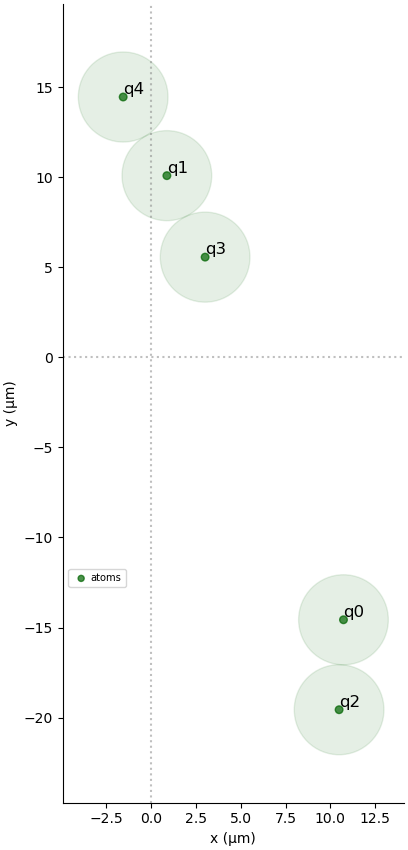
\includegraphics[width=0.4\textwidth]{img/embedding/reg_5x5_SA.png} 
    \caption{The 2D physical spatial layout generated by the enhanced Simulated Annealing engine for the $N=5$ instance. The register fully complies with Neutral Atom QPU geometric boundaries.}
    \label{fig:5x5_register_SA}
\end{figure}

An interesting geometric observation emerges when comparing this layout to the one produced by the GA. While the absolute continuous spatial coordinates differ significantly from the ones generated in the previous chapter, the underlying structural topology and the isolation of the logical sub-graphs remain perfectly isomorphic.

In figure \ref{fig:5x5_quantum_res_SA}, the quantum execution results are reported:

\begin{figure}[H]
    \centering
    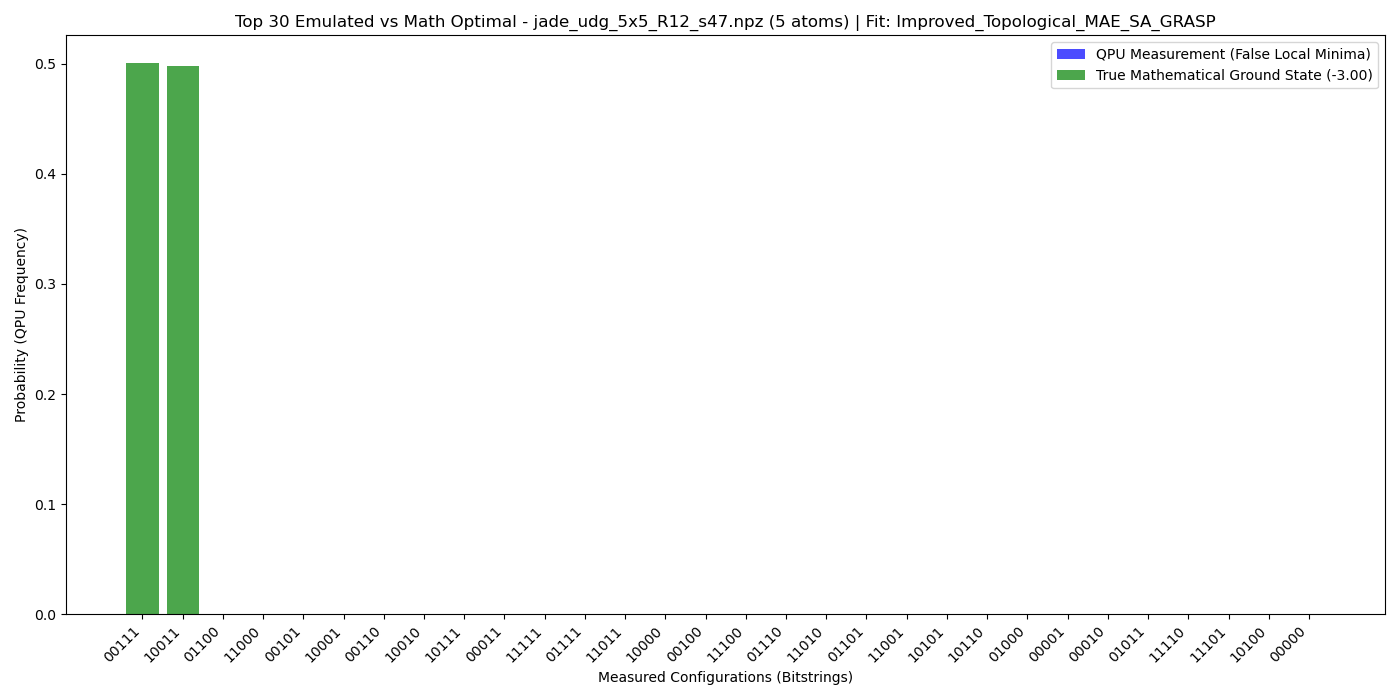
\includegraphics[width=1.0\textwidth]{img/res/res_5x5_SA.png} 
    \caption{Probability distribution of the measured bitstrings after the adiabatic execution on the QPU emulator. The highest probability peaks correspond perfectly to the optimal solutions of the original QUBO instance.}
    \label{fig:5x5_quantum_res_SA}
\end{figure}

The dominant probability mass and the perfect symmetry of the peaks clearly highlight the successful identification of the global mathematical optima. Consequently, the SA-enhanced embedding pipeline is formally validated for small-scale instances, providing a solid and reliable baseline for the subsequent scaling stress-tests.


\section{Scaling Up: The $10\times10$ Instance}

Moving on to the operational limit instance that severely hindered the Genetic Algorithm, previously formalized in Figure \ref{fig:10x10_qubo_instance}, we applied the thermodynamic parametrization detailed in Table \ref{tab:sa_parameters_10x10}.

\begin{table}[H]
    \centering
    \renewcommand{\arraystretch}{1.3}
    \resizebox{\textwidth}{!}{
    \begin{tabular}{l c p{0.55\textwidth}}
        \hline
        \textbf{SA Parameter} & \textbf{Configured Value} & \textbf{Conceptual Meaning} \\
        \hline
        \texttt{num\_restarts} & $10$ & Multi-start execution approach. The algorithm is independently restarted to mitigate stochastic initialization, selecting the absolute minimum energy state found. \\
        \texttt{T\_INIT} & $50000.0$ & Initial Temperature. Purposely set extremely high to allow the algorithm to freely explore the continuous spatial search space during the early phases. \\
        \texttt{T\_MIN} & $0.1$ & Minimum Temperature (Stopping Criterion). The threshold at which the system freezes before the final Quenching phase begins. \\
        \texttt{COOLING\_RATE} & $0.99$ & The exponential decay factor applied to the temperature after each thermodynamic cycle ($T = T \times 0.99$). Increased to guarantee an even slower and more meticulous cooling process for the denser graph. \\
        \texttt{STEPS\_PER\_TEMP} & $1000$ & Markov Chain length. The number of neighboring geometric configurations generated and evaluated at each discrete temperature level. \\
        \hline
    \end{tabular}
    }
    \caption{Specific hyperparameter configuration for the Simulated Annealing engine adopted for the $10\times10$ instance evaluation, as extracted from the experimental registry.}
    \label{tab:sa_parameters_10x10}
\end{table}

This aggressive and heavily cooled execution yielded a spatial fitness score of $0.1261$, requiring a classical execution time of $2417.55$ seconds. When compared to the Genetic Algorithm's performance on this exact same matrix (which struggled to achieve a fitness score of $0.0583$ in $1408.8$ seconds, as documented in Section 4.4), the Simulated Annealing engine delivered a topological mapping quality more than twice as accurate. Regarding the extended computational execution time, all the considerations previously outlined for the $5\times5$ instance remain valid: the classical overhead is a direct consequence of the rigorous $10$-restart multi-shot approach combined with the prolonged cooling schedule, deliberately chosen to prioritize absolute geometric precision over optimization speed. 

This meticulous thermodynamic search resulted in the spatial embedding illustrated in Figure \ref{fig:10x10_register_SA}.

\begin{figure}[H]
    \centering
    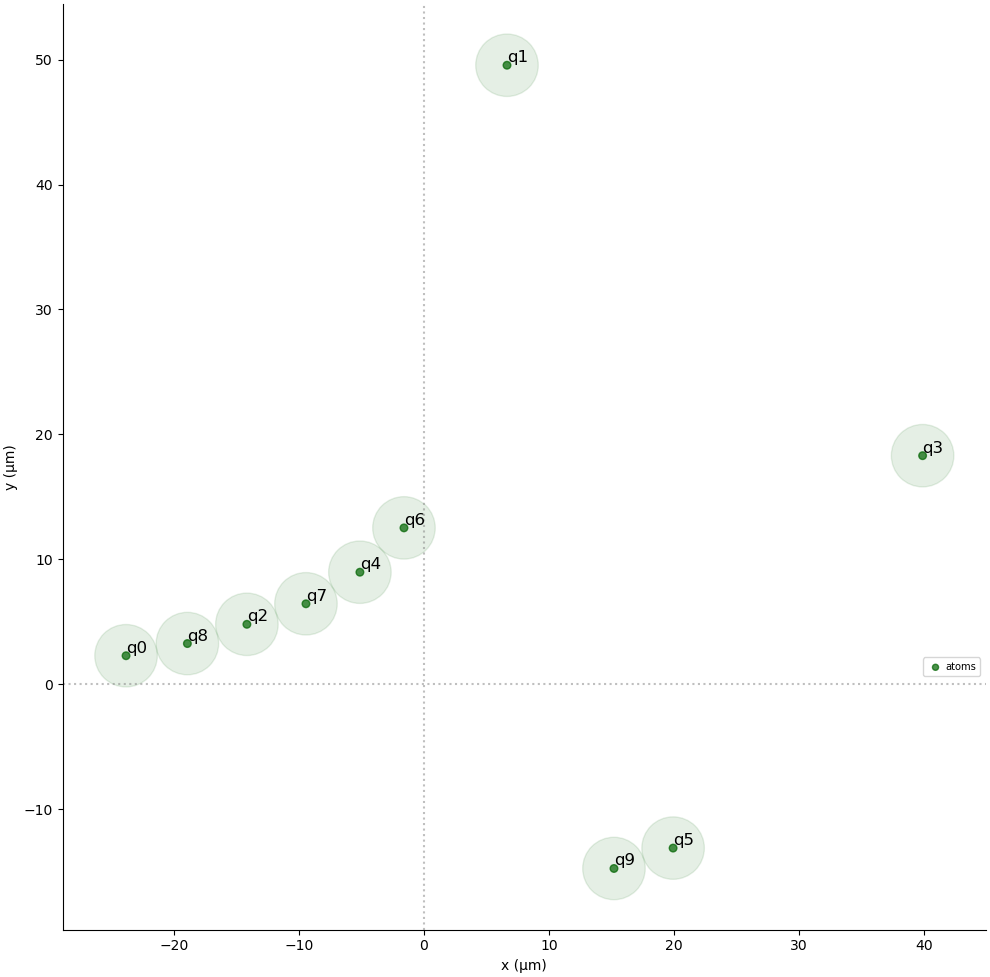
\includegraphics[width=0.6\textwidth]{img/embedding/reg_10x10_SA.png} 
    \caption{The 2D physical spatial layout generated by the enhanced Simulated Annealing engine for the $N=10$ instance. The register fully complies with Neutral Atom QPU geometric boundaries.}
    \label{fig:10x10_register_SA}
\end{figure}

The physical layout demonstrates remarkable structural clarity: the central chain structure, accompanied by localized isolated atomic pairs (islands), is perfectly defined. Unlike the GA, which struggled to balance density and hardware boundaries at this scale, the SA engine successfully shaped the complex topological constraints without triggering any catastrophic spatial overlaps.

To definitively prove the validity of this embedding, the generated physical coordinates were mapped into the standard adiabatic sequence and submitted to the quantum emulator, producing the measurement distribution reported in Figure \ref{fig:10x10_quantum_res_SA}.

\begin{figure}[H]
    \centering
    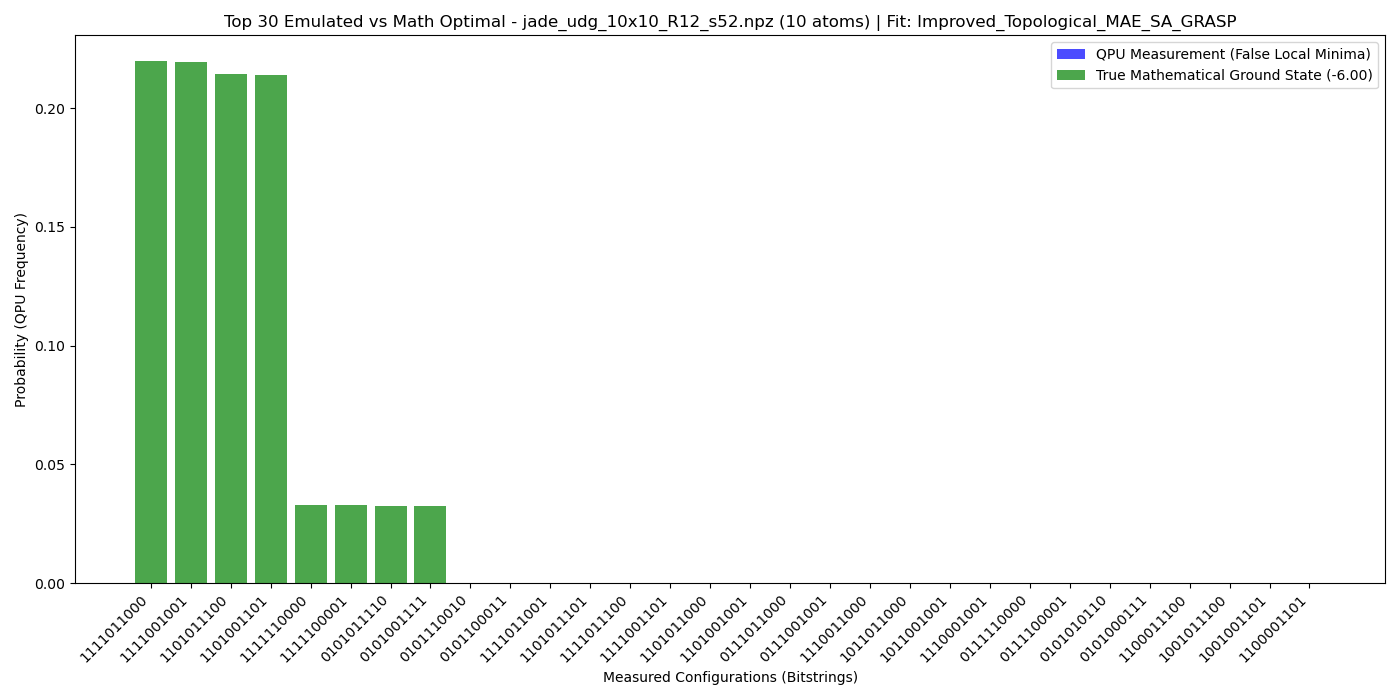
\includegraphics[width=1.0\textwidth]{img/res/res_10x10_SA.png} 
    \caption{Probability distribution of the measured bitstrings after the adiabatic execution on the QPU emulator. The highest probability peaks correspond perfectly to the optimal solutions of the original QUBO instance.}
    \label{fig:10x10_quantum_res_SA}
\end{figure}

As is evident from the histogram, the quantum execution flawlessly identified the true mathematical ground states with a prominent and symmetric probability mass. This result confirms that the GRASP-enhanced Simulated Annealing efficiently overcomes the dimensionality bottleneck that previously compromised the evolutionary pipeline at the $N=10$ scale.

\section{Overcoming the Bottleneck: The $15\times15$ Instance}

This instance represents the critical juncture where the GRASP-enhanced Simulated Annealing definitively outperforms the Genetic Algorithm, highlighting highly promising scaling dynamics. The target QUBO problem is the exact same $N=15$ configuration that caused the complete breakdown of the evolutionary pipeline, previously depicted in Figure \ref{fig:15x15_qubo_instance}. 

To tackle this matrix, the SA engine was executed using the parameter configuration detailed in Table \ref{tab:sa_parameters_15x15}.

\begin{table}[H]
    \centering
    \renewcommand{\arraystretch}{1.3}
    \resizebox{\textwidth}{!}{
    \begin{tabular}{l c p{0.55\textwidth}}
        \hline
        \textbf{SA Parameter} & \textbf{Configured Value} & \textbf{Conceptual Meaning} \\
        \hline
        \texttt{num\_restarts} & $10$ & Multi-start execution approach. The algorithm is independently restarted to mitigate stochastic initialization, selecting the absolute minimum energy state found. \\
        \texttt{T\_INIT} & $50000.0$ & Initial Temperature. Purposely set extremely high to allow the algorithm to freely explore the continuous spatial search space during the early phases. \\
        \texttt{T\_MIN} & $0.1$ & Minimum Temperature (Stopping Criterion). The threshold at which the system freezes before the final Quenching phase begins. \\
        \texttt{COOLING\_RATE} & $0.99$ & The exponential decay factor applied to the temperature after each thermodynamic cycle ($T = T \times 0.99$). \\
        \texttt{STEPS\_PER\_TEMP} & $1000$ & Markov Chain length. The number of neighboring geometric configurations generated and evaluated at each discrete temperature level. \\
        \hline
    \end{tabular}
    }
    \caption{Specific hyperparameter configuration for the Simulated Annealing engine adopted for the $15\times15$ instance evaluation, as extracted from the experimental registry. The configuration remains strictly identical to the $10\times10$ setup, highlighting the superior intrinsic scalability of the thermodynamic heuristic.}
    \label{tab:sa_parameters_15x15}
\end{table}

Notably, the thermodynamic hyperparameters remain strictly identical to those used for the $10\times10$ instance. This suggests that either the SA engine possesses a superior intrinsic scaling capacity, or the previous configuration was conservatively over-parameterized. Regardless, it demonstrates a robust degree of algorithmic flexibility, eliminating the need for the exhaustive manual retuning and exponential computational inflation that was mandatory for the GA.

This configuration generated the physical embedding illustrated in Figure \ref{fig:15x15_register_SA}.

\begin{figure}[H]
    \centering
    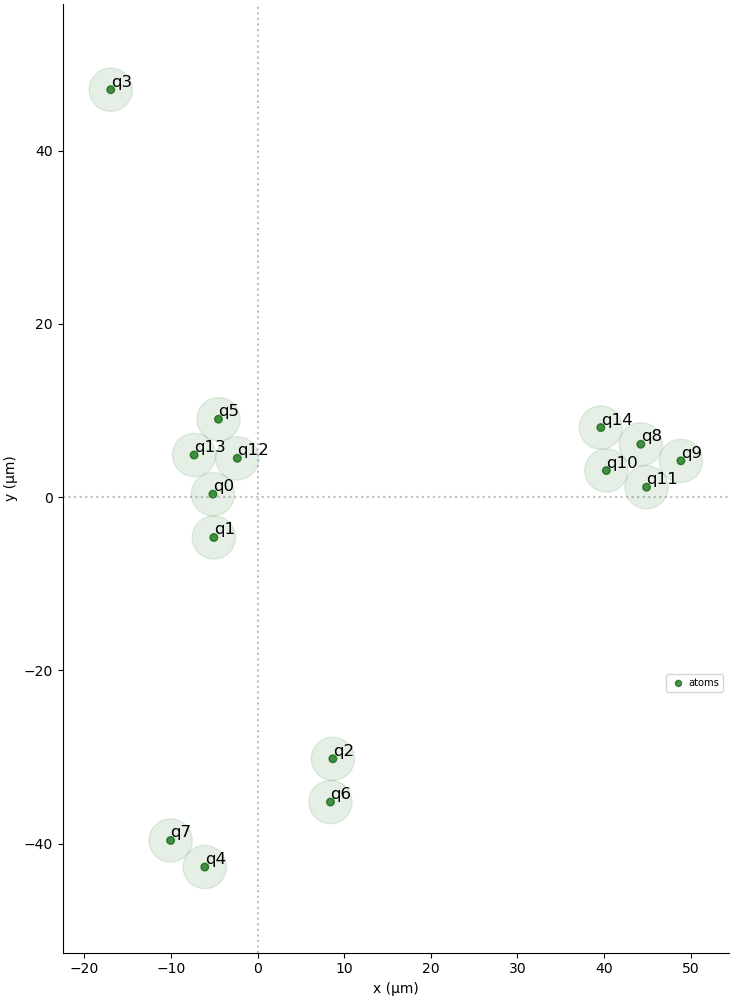
\includegraphics[width=0.\textwidth]{img/embedding/reg_15x15_SA.png} 
    \caption{The 2D physical spatial layout generated by the enhanced Simulated Annealing engine for the $N=15$ instance. The register fully complies with Neutral Atom QPU geometric boundaries.}
    \label{fig:15x15_register_SA}
\end{figure}

The classical execution required $2429.1$ seconds, yielding a spatial fitness score of $0.04305$. While this fitness score is numerically lower than those achieved on smaller grids, it is nearly six times higher than the $0.0075$ score produced by the GA on this same matrix. This topological superiority is unequivocally confirmed by the quantum simulation readout in Figure \ref{fig:15x15_quantum_res_SA}.

\begin{figure}[H]
    \centering
    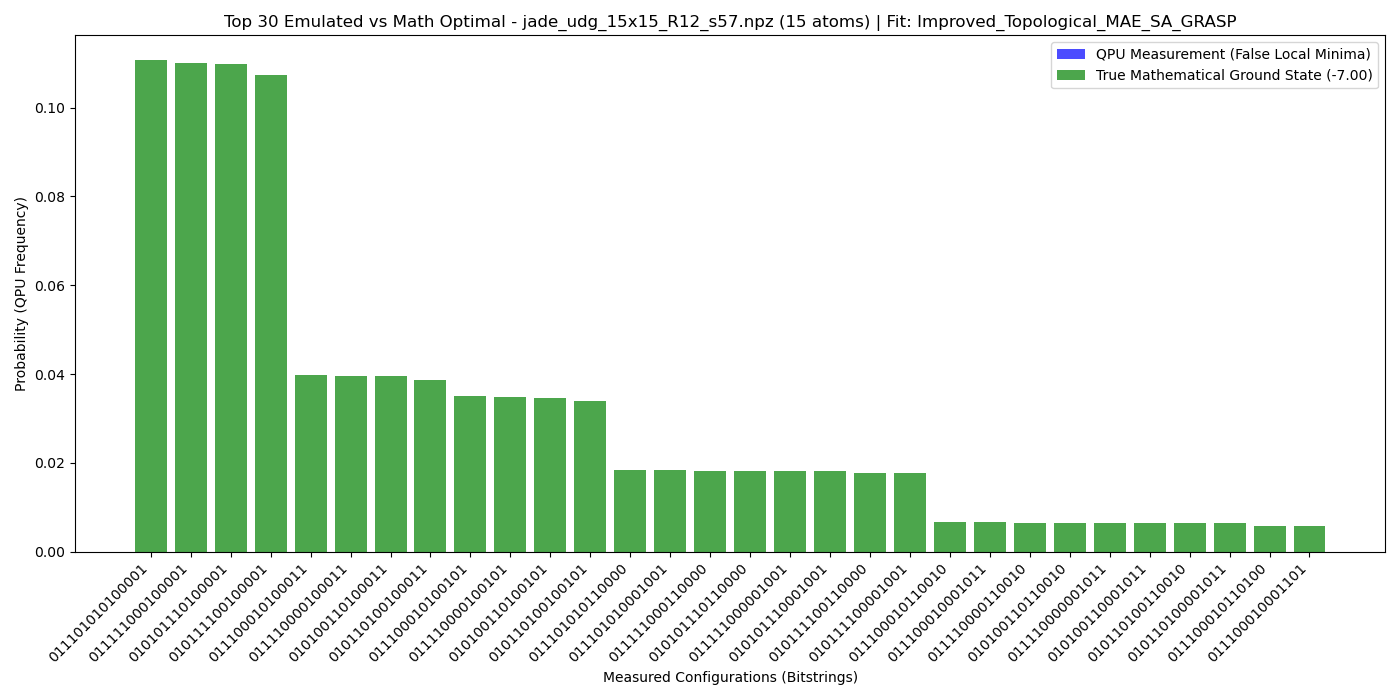
\includegraphics[width=1.0\textwidth]{img/res/res_15x15_SA.png} 
    \caption{Probability distribution of the measured bitstrings after the adiabatic execution on the QPU emulator. The highest probability peaks correspond perfectly to the optimal solutions of the original QUBO instance.}
    \label{fig:15x15_quantum_res_SA}
\end{figure}

Unlike the GA pipeline, which failed to identify any valid ground state on this problem, the analog simulation successfully isolated the multiple degenerate optimal solutions with a dominant probability mass (peaking at approximately $11.07\%$). 

Drawing preliminary conclusions from this comparative analysis, we can affirm that the GRASP-enhanced Simulated Annealing exhibits vastly superior scaling capabilities. Crucially, its classical computational overhead is primarily dictated by the explicit thermodynamic parametrization rather than suffering the immediate, exponential explosion triggered by problem dimensionality observed in Genetic Algorithms. Ultimately, this validates the overall robustness and efficacy of our hybrid classical-quantum pipeline when driven by a specialized SA embedding engine.

Having secured this algorithmic victory, the natural progression of our analysis leads to a fundamental question: to what extent can this SA pipeline scale before it, too, encounters the physical and computational limits of the neutral atom architecture?

\section{Scaling Up: The $20\times20$ Instance}
\label{sec:scaling_20x20}

The $20\times20$ matrix represents the final dimensional scale tested in our direct embedding approach. Going beyond this threshold causes the classical simulation time required by the remote HPC infrastructure to skyrocket from minutes or hours to days. This simulator-imposed limit does not imply a physical impossibility of embedding larger instances on real hardware. Instead, it simply sets a realistic experimental boundary for our research. We selected this specific dimension as the best possible trade-off among geometric complexity, classical preprocessing time, and quantum emulation overhead. Setting this limit also serves a highly practical purpose for this thesis: it creates the perfect baseline to introduce our \textit{Divide et Impera} (divide and conquer) approach. After all, in real-world scenarios, both hardware availability and quantum emulation capacities are often constrained by a limited number of qubits. This makes the $20\times20$ scale a very credible and representative benchmark.

The mathematical formulation of this target instance is shown in Figure \ref{fig:20x20_qubo_instance}.

\begin{figure}[htbp]
    \centering
    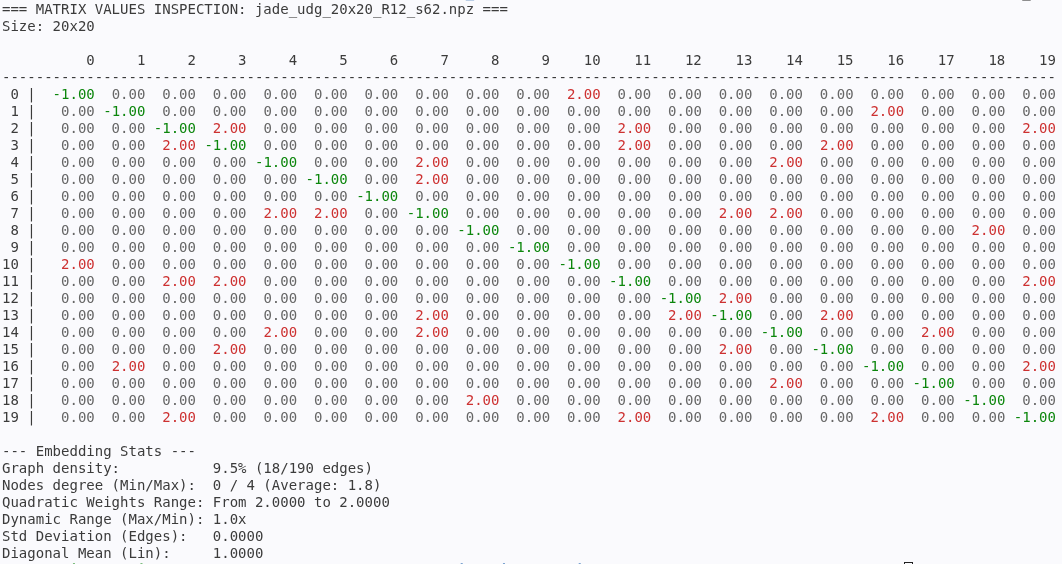
\includegraphics[width=0.8\textwidth]{img/QUBO_instances/20x20_r12_s62_d3.0.png} 
    \caption{Structure of the $20 \times 20$ UDG-like QUBO instance generated via \textit{instance\_generator.py}, inspected using \textit{inspect\_qubo.py}, and subsequently embedded using the \textit{bench-SA.py} module \cite{orsucci_qubo_ga_quantum}.}
    \label{fig:20x20_qubo_instance}
\end{figure}

With an instance of this size, traditional classical heuristics begin to hit a computational wall. The continuous search space expands dramatically. Coupled with a moderate density and a non-trivial maximum node degree, the geometric difficulty becomes severe. To handle this combinatorial challenge, we configured the SA engine with the parameters detailed in Table \ref{tab:sa_parameters_20x20}.

\begin{table}[H]
    \centering
    \renewcommand{\arraystretch}{1.3}
    \resizebox{0.65\textwidth}{!}{
    \begin{tabular}{l c p{0.55\textwidth}}
        \hline
        \textbf{SA Parameter} & \textbf{Configured Value} & \textbf{Conceptual Meaning} \\
        \hline
        \texttt{num\_restarts} & $15$ & Massive multi-start execution approach. Increased from $10$ to $15$ to aggressively counteract the stochastic nature of the algorithm over the vastly expanded continuous geometric space of 20 atoms. \\
        \texttt{T\_INIT} & $50000.0$ & Initial Temperature. Kept extremely high to allow the algorithm to overcome massive early-stage hardware penalties (100k) and freely explore the space. \\
        \texttt{T\_MIN} & $0.1$ & Minimum Temperature (Stopping Criterion). The threshold at which the system freezes before the final Quenching phase begins. \\
        \texttt{COOLING\_RATE} & $0.99$ & The exponential decay factor applied to the temperature after each thermodynamic cycle. Functions as an extremely slow cooling schedule for densely constrained layouts. \\
        \texttt{STEPS\_PER\_TEMP} & $2000$ & Markov Chain Monte Carlo (MCMC) steps per epoch. Doubled compared to the $15\times15$ instance (from $1000$ to $2000$) to guarantee a much deeper spatial exploration at each discrete temperature level. \\
        \hline
    \end{tabular}
    }
    \caption{Extreme hyperparameter configuration for the Simulated Annealing engine adopted for the $20\times20$ instance evaluation. The parametrization highlights a "brute-force" approach to overcome the "curse of dimensionality", heavily increasing both the number of restarts and the MCMC iterations per thermal epoch.}
    \label{tab:sa_parameters_20x20}
\end{table}

This specific setup relies on what we can define a \textit{thermodynamic brute-force} strategy. The parameters are intentionally aggressive. By forcing $15$ restarts and $2000$ thermal steps, we push the algorithm to exhaustively explore a massive landscape of local minima. Because of this, the classical execution took $7669.73$ seconds (just over two hours) and achieved a spatial fitness score of $0.0102$. The classical overhead is obviously substantial, limited by the hardware specifications reported in Appendix \ref{app:hardware_specs}. Even so, the algorithm successfully converged into a valid topological configuration, leading to the physical embedding shown in Figure \ref{fig:20x20_register_SA_d3.0}.

\begin{figure}[H]
    \centering
    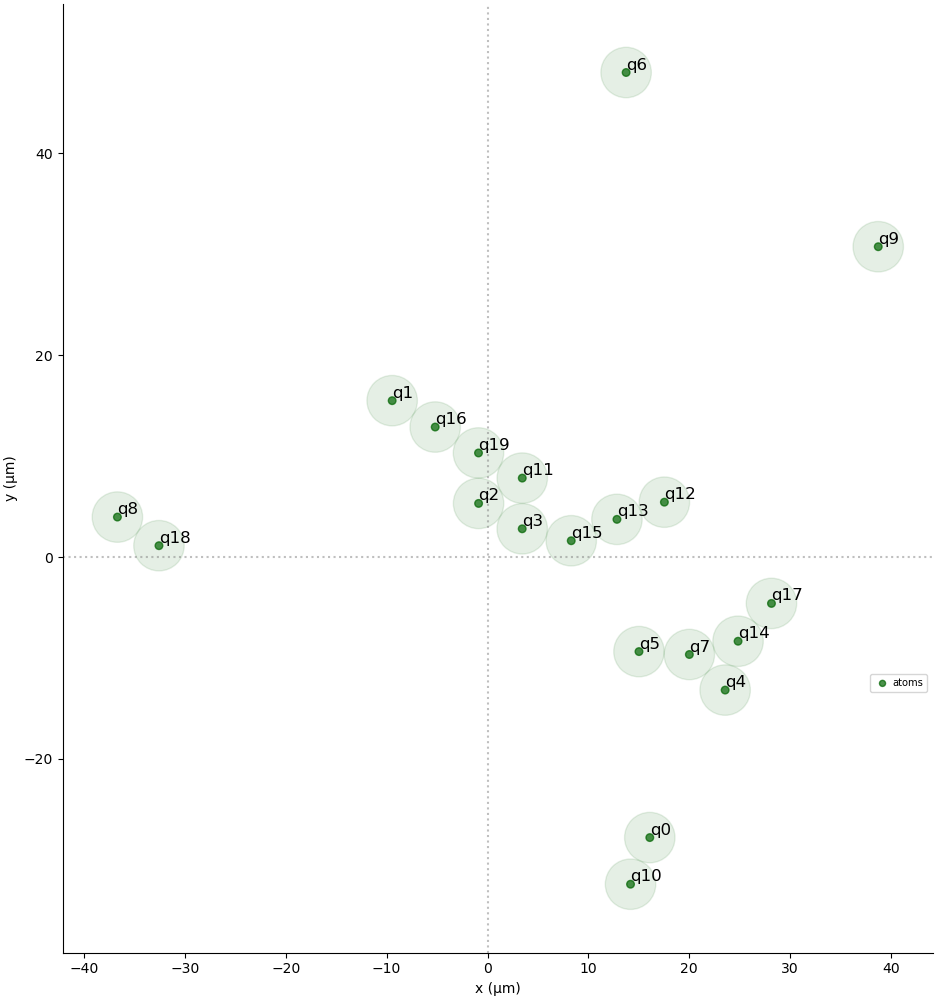
\includegraphics[width=0.6\textwidth]{img/embedding/reg_20x20_d3.0.png} 
    \caption{The 2D physical spatial layout generated by the enhanced Simulated Annealing engine for the $N=20$ instance. The register fully complies with Neutral Atom QPU geometric boundaries.}
    \label{fig:20x20_register_SA_d3.0}
\end{figure}

To verify the validity of this layout, we mapped the generated coordinates into the quantum emulator. The resulting statistical distribution is reported in Figure \ref{fig:20x20_quantum_res_SA_d3.0}.

\begin{figure}[H]
    \centering
    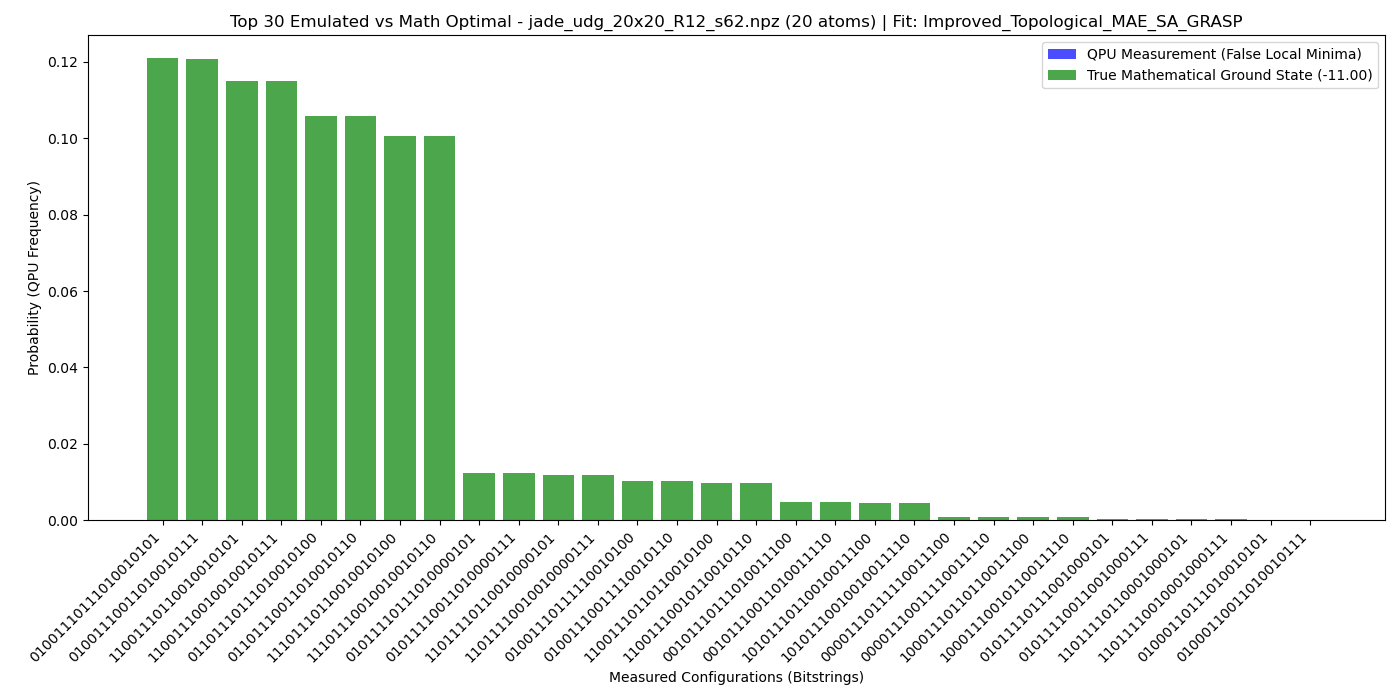
\includegraphics[width=1.0\textwidth]{img/res/res_20x20_d3.0.png} 
    \caption{Probability distribution of the measured bitstrings after the adiabatic execution on the QPU emulator. The highest probability peaks correspond perfectly to the optimal solutions of the original QUBO instance.}
    \label{fig:20x20_quantum_res_SA_d3.0}
\end{figure}

The histogram speaks clearly: if provided with a deep enough thermodynamic parametrization, the Simulated Annealing engine scales successfully up to a $20\times20$ QUBO instance and effectively isolates the mathematical ground states. This result proves once again the analog resilience of the Neutral Atom platform: a mathematically sub-optimal spatial fitness is still perfectly capable of guiding the quantum dynamics toward the correct solution.

We ran several other supplementary experiments on matrices characterized by different densities and node degrees, but for the sake of brevity, we chose to report only the following specific instance, as the main conclusions drawn from these scaling tests remain exactly the same.


\section{A Denser $20\times20$ Instance}
\label{sec:denser_20x20}

To further investigate the algorithmic breaking point, we tested a distinct $20\times20$ target instance characterized by a significantly higher geometric density. The mathematical structure of this specific UDG-like QUBO matrix is presented in Figure \ref{fig:20x20_qubo_instance_d5}.

\begin{figure}[htbp]
    \centering
    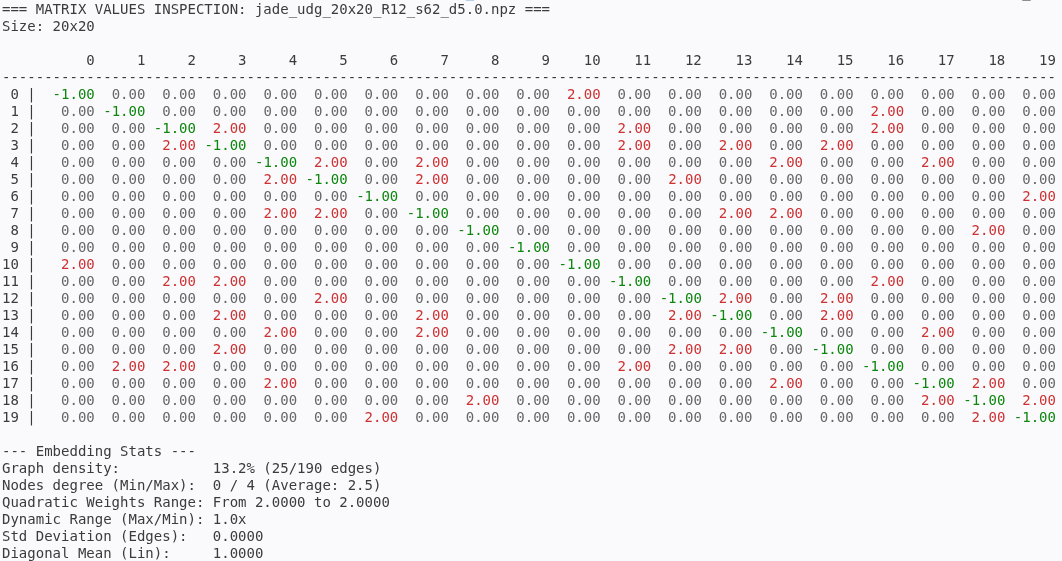
\includegraphics[width=0.8\textwidth]{img/QUBO_instances/20x20_r12_s62_d5.0.png} 
    \caption{Structure of the denser $20 \times 20$ UDG-like QUBO instance generated via \textit{instance\_generator.py}, inspected using \textit{inspect\_qubo.py}, and subsequently embedded using the \textit{bench-SA.py} module \cite{orsucci_qubo_ga_quantum}.}
    \label{fig:20x20_qubo_instance_d5}
\end{figure}

Due to the increased interplay and node degree, applying the previous brute-force exploration would have caused an unsustainable explosion in classical execution times. Therefore, we shifted toward a highly conservative parameterization designed to strictly preserve the initial deterministic geometric configuration generated by the GRASP pre-placer. This specific setup is detailed in Table \ref{tab:sa_parameters_20x20_d5}.

\begin{table}[H]
    \centering
    \renewcommand{\arraystretch}{1.3}
    \begin{tabularx}{\textwidth}{l c X}
        \hline
        \textbf{SA Parameter} & \textbf{Configured Value} & \textbf{Conceptual Meaning} \\
        \hline
        \texttt{num\_restarts} & $15$ & Massive multi-start execution. Maintained at 15 to counteract stochastic initialization over the dense 20-node search space. \\
        \texttt{T\_INIT} & $50.0$ & Initial Temperature. Drastically reduced (from $50000.0$) to prevent the algorithm from destroying the initial geometry generated by the GRASP pre-placer, focusing strictly on localized topological fine-tuning. \\
        \texttt{T\_MIN} & $0.01$ & Minimum Temperature. Lowered to force a much deeper thermodynamic freeze before initiating the final Quenching sequence. \\
        \texttt{COOLING\_RATE} & $0.98$ & The exponential decay factor applied to the temperature after each thermodynamic cycle. \\
        \texttt{STEPS\_PER\_TEMP} & $800$ & Markov Chain length. Significantly reduced (from $2000$) to cap the exponential growth of the classical computational time. \\
        \hline
    \end{tabularx}
    \caption{Specific hyperparameter configuration adopted for the denser $20\times20$ instance (\texttt{d5.0}). This parameter tuning shifts away from brute-force exploration, heavily relying on the GRASP initialization to contain the classical computational execution time.}
    \label{tab:sa_parameters_20x20_d5}
\end{table}

By relying on this conservative thermodynamic approach, the classical execution required $2125.04$ seconds. While the computational time was successfully contained, the spatial constraint satisfaction suffered heavily, yielding a poor spatial fitness score of $0.0039$. Despite this low mathematical accuracy, the algorithm managed to generate the physically valid embedding shown in Figure \ref{fig:20x20_register_SA_d5.0}.

\begin{figure}[H]
    \centering
    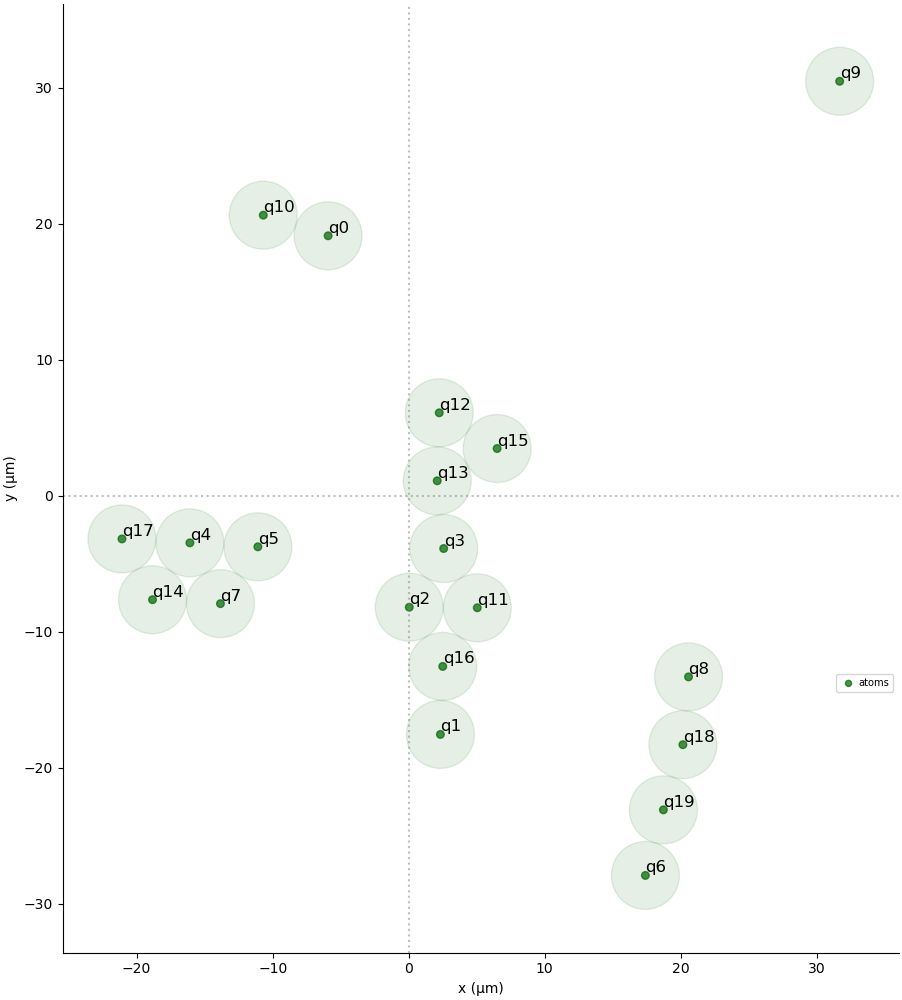
\includegraphics[width=0.6\textwidth]{img/embedding/reg_20x20_d5.0_third.png} 
    \caption{The 2D physical spatial layout generated by the enhanced Simulated Annealing engine for the denser $N=20$ instance. The register fully complies with Neutral Atom QPU geometric boundaries.}
    \label{fig:20x20_register_SA_d5.0}
\end{figure}

To evaluate the actual impact of this degraded spatial quality, the layout was validated through the analog quantum emulator. The measurement readout is reported in Figure \ref{fig:20x20_quantum_res_SA_d5.0}.

\begin{figure}[H]
    \centering
    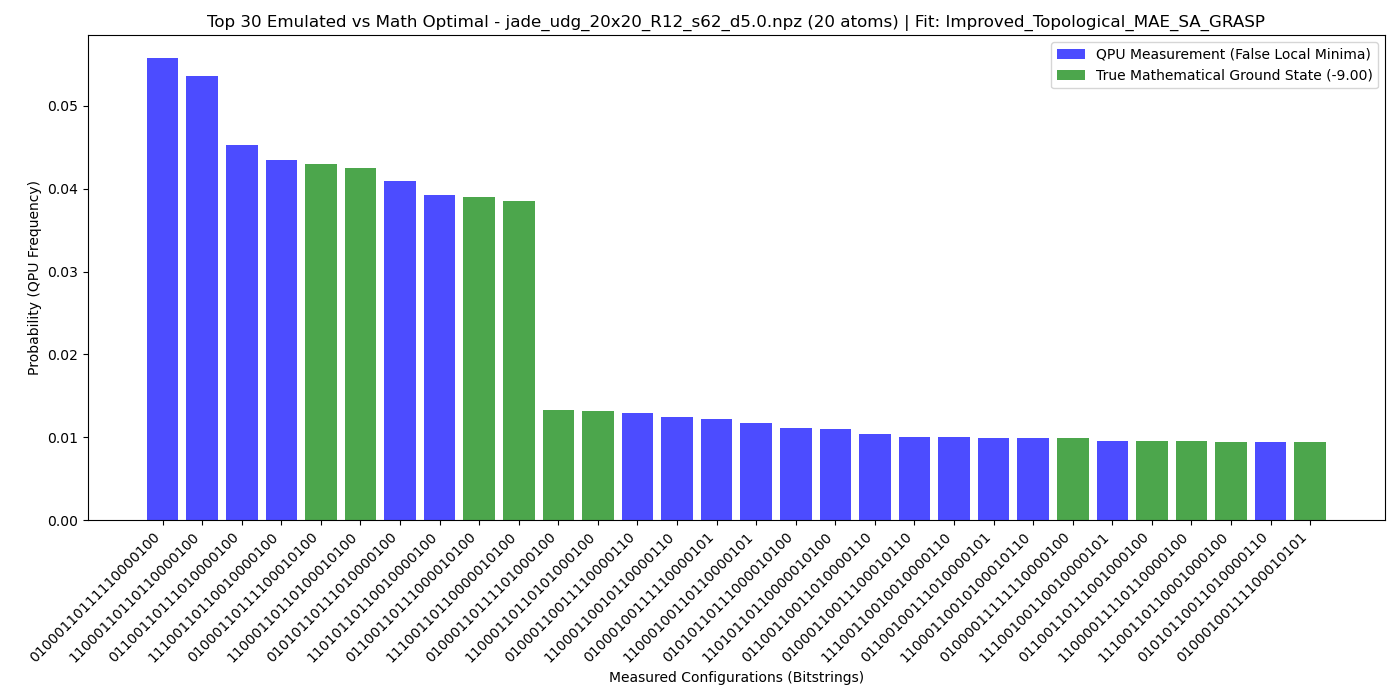
\includegraphics[width=1.0\textwidth]{img/res/res_20x20_d5.0_third.png} 
    \caption{Probability distribution of the measured bitstrings after the adiabatic execution on the QPU emulator. While noisy, the system managed to identify at least one optimal solution of the original QUBO instance.}
    \label{fig:20x20_quantum_res_SA_d5.0}
\end{figure}

Unlike previous test cases, we no longer observe a perfectly symmetric probability mass or pristine high-quality peaks. The quantum distribution is noticeably noisier and less dominant. Nevertheless, the analog execution still successfully identified at least one global mathematical optimum.

Ultimately, this dense $20\times20$ instance exposes the operational breaking point of our baseline pipeline. While the embedding approach remains technically effective, the severe loss in spatial fitness and the consequent degradation of the quantum readout demonstrates clear scalability limitations dictated by the sheer size and density of the problem. It becomes unequivocally evident that directly tackling larger or denser matrices using a monolithic, single-core classical heuristic is no longer computationally viable. To efficiently overcome this bottleneck and process complex layouts in a manageable timeframe, a paradigm shift is strictly required. This lays the definitive groundwork for the introduction of our \textit{Divide et Impera} architecture.
